%% ---------------------------------------------------------------------------------------------------------
\section{A second policy architecture}\label{sec:generalization}

\paragraph{Question} Is the gain specific to the two ResNet-18 policies, which share architecture and data and differ only in the training seed? This stage is development-level: one pre-declared test, no calibration.

\begin{figure}[!htbp]
\centering
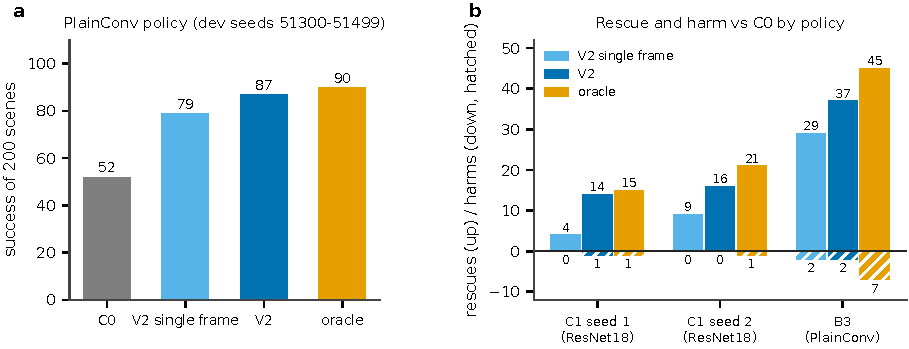
\includegraphics[width=\linewidth]{Fig09_generalization_plainconv.pdf}
\caption{Unchanged V2 on a frozen policy of a different architecture (PlainConv encoder; development seeds 51300--51499; same task and demonstrations). (a) Successes of 200 scenes. (b) Rescues (up) and harms (down, hatched) against C0 for the two ResNet-18 development policies and the PlainConv policy.}\label{fig:gen}
\end{figure}

\begin{table}[!htbp]
\centering\footnotesize
\caption{PlainConv policy, development level (200 scenes; two-sided 95\% Clopper--Pearson intervals, descriptive).}\label{tab:gen}
\input{\tabdir T6_generalization_plainconv.tex}
\end{table}

\paragraph{Evidence} Applied without any change to a frozen policy with a weaker, non-pretrained encoder, V2 raised success from 52 to 87 of 200 scenes, with 37 rescues and 2 harms ($p=1.4\times10^{-9}$, the single pre-declared test; Table~\ref{tab:gen}, Fig.~\ref{fig:gen}). It recovered 37 of the 45 oracle rescues; the oracle itself caused 7 harms. The single-frame variant reached 79 (29 rescues, 2 harms).

\paragraph{Interpretation and limits} The same release-time offset is a frequent failure of the weaker policy, and at development level V2 corrects many of these failures without retuning. There is no calibration certificate for this policy: its 2 harms among 52 baseline successes (3.8\%) are not a bound. The policies share the task and the demonstrations, so this is not evidence of transfer to other tasks.
